%! Author = jonathan
%! Date = 6/1/24

\documentclass[a0paper,portrait]{baposter}

\usepackage{lmodern}
%\usepackage[lining]{sourcesanspro} Typeface for Cornell Bowers CIS
\usepackage[export]{adjustbox}
\usepackage[utf8]{inputenc}
\usepackage{colortbl}
\usepackage{arydshln}
\usepackage{booktabs}
\usepackage{forest}
\usepackage{tcolorbox}
\usepackage{multicol}
\usepackage[font=small,labelfont=bf]{caption}
\usepackage{multirow}
\usepackage[
    backend=biber,
    style=numeric,
    sorting=ynt,
    maxnames=1,
    doi=false,
    isbn=false,
    url=false,
    eprint=false
]{biblatex}
\addbibresource{main.bib}
\DeclareNameFormat{family}{% https://tex.stackexchange.com/a/529305
    \usebibmacro{name:family}
    {\namepartfamily}
    {\namepartgiven}
    {\namepartprefix}
    {\namepartsuffix}%
    \usebibmacro{name:andothers}}

\DeclareNameAlias{default}{family}

\newcommand{\methodname}{Aristos}

\newcommand{\compresslist}{
    \setlength{\itemsep}{0pt}
    \setlength{\parskip}{1pt}
    \setlength{\parsep}{0pt}
}

\newenvironment{boenumerate}
{\begin{enumerate}\renewcommand\labelenumi{\textbf\theenumi.}}
{\end{enumerate}}

\definecolor{mygray}{RGB}{226, 226, 226}
\definecolor{myred}{RGB}{252, 142, 142}
\definecolor{mygreen}{RGB}{147, 255, 143}
\definecolor{myblue}{RGB}{144, 155, 255}
\definecolor{myyellow}{RGB}{253, 253, 143}
\definecolor{mypurple}{RGB}{255, 142, 250}

\definecolor{bordercolor}{RGB}{248,152,29}
\definecolor{backgroundcolor}{RGB}{0,102,153}
\captionsetup{justification=raggedright,singlelinecheck=false} %https://tex.stackexchange.com/a/275141
\begin{document}
    \begin{poster}
    {
        grid=false,
        headerborder=open, % Adds a border around the header of content boxes
        colspacing=1em, % Column spacing
        bgColorOne=white, % Background color for the gradient on the left side of the poster
        bgColorTwo=white, % Background color for the gradient on the right side of the poster
        borderColor=bordercolor, % Border color
        headerColorOne=backgroundcolor, % Background color for the header in the content boxes (left side)
        headerColorTwo=backgroundcolor, % Background color for the header in the content boxes (right side)
        headerFontColor=white, % Text color for the header text in the content boxes
        boxColorOne=white, % Background color of the content boxes
        textborder=rounded, %rectangle, % Format of the border around content boxes, can be: none, bars, coils, triangles, rectangle, rounded, roundedsmall, roundedright or faded
        eyecatcher=false, % Set to false for ignoring the left logo in the title and move the title left
        headerheight=0.11\textheight, % Height of the header
        headershape=rounded, % Specify the rounded corner in the content box headers, can be: rectangle, small-rounded, roundedright, roundedleft or rounded
        headershade=plain,
        headerfont=\Large\textsf, % Large, bold and sans serif font in the headers of content boxes
        %textfont={\setlength{\parindent}{1.5em}}, % Uncomment for paragraph indentation
        linewidth=2pt, % Width of the border lines around content boxes
        authorfont=\large\sffamily\mdseries\setlength\baselineskip{2.2ex}, %https://tex.stackexchange.com/a/7670
        titlefont=\sffamily\bfseries\Huge\setlength{\baselineskip}{2.2ex}%
    }

%
%-----------------------------
%	TITLE AND AUTHOR NAME
%-----------------------------
%
    {
%        \vspace{0.25em}
        Aristos: Pipelining One-sided \\ Communication in Distributed \\ Mixture of Experts (MoE)
    }
    {
        \vspace{-0.1em}
        \textbf{Osayamen Jonathan Aimuyo}$^{\dagger}$\vspace{0.1em}\\%
        \small{\texttt{oja7@cornell.edu} \; $^{\dagger}$
            \textit{Cornell Ann S. Bowers College of Computing and Information Science, Cornell University}}
        \vspace{-1.1em}
    }
    {
        
\includegraphics[width=8.5cm,keepaspectratio]{figures/cornell}
    }


        \headerbox{Background}{name=prelim,span=1,column=0}{
            \begin{center}
                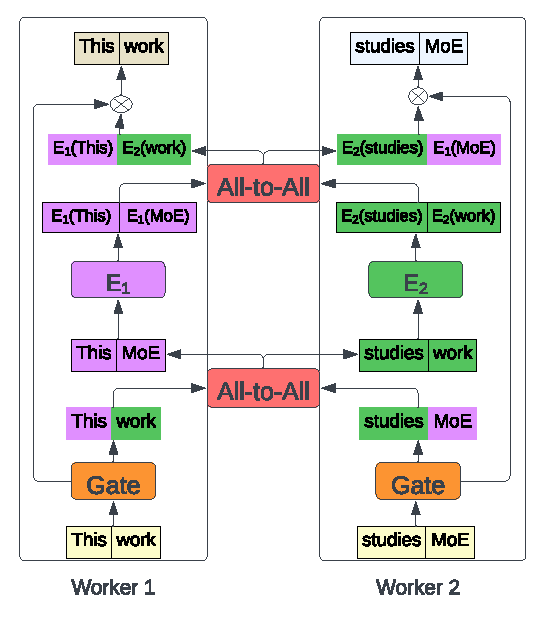
\includegraphics[width=7cm,keepaspectratio, left]{figures/moe_only}
            \captionof{figure}{
                \footnotesize{DMoE with $W = EP = 2$.
                The \textbf{Gate} routes tokens to experts;
                    \textbf{All-to-All} disseminates tokens; expert/\textbf{FFN} computation occurs;
                    \textbf{All-to-All} reconsitutes tokens followed by the~\textbf{Scale} computation.}}
            \end{center}
        }

        \headerbox{Challenges}{name=challenges,span=2,column=1}{
                \footnotesize{The widely-adopted~\cite{dbrx} MoE architecture,
                    promising \textbf{5x} faster training and
            \textbf{9x} reduced inference costs~\cite{pmlr-v162-rajbhandari22a}, is currently plagued by
            three \textit{open} challenges~\cite{deep_comm, 10.1145/3603269.3604869, JMLR:v23:21-0998}
                    in the distributed setting.}
            \begin{center}
                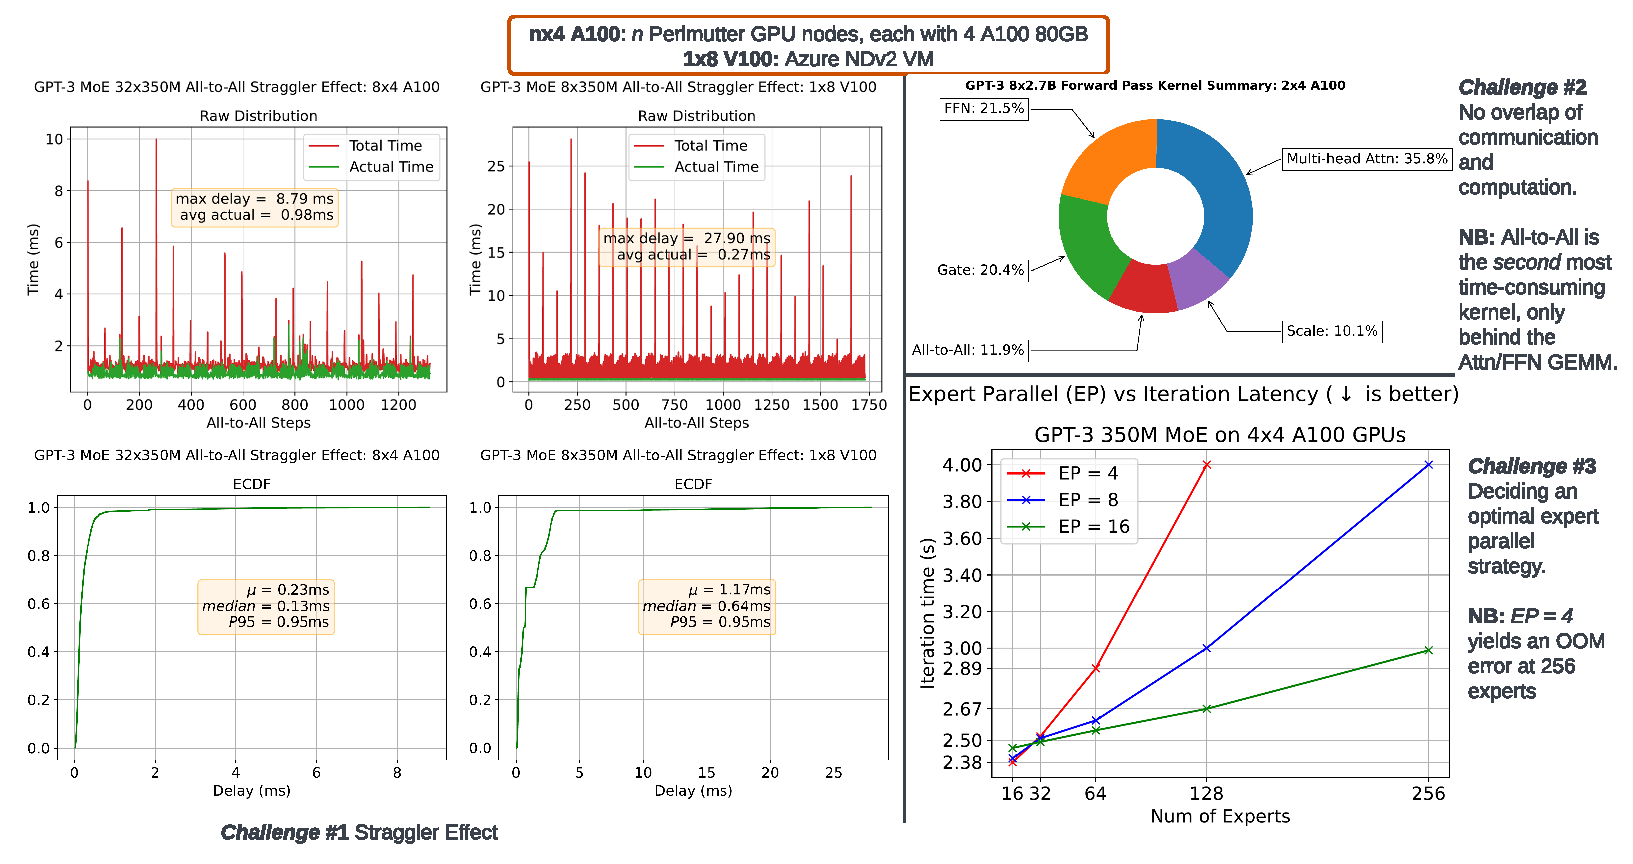
\includegraphics[width=15.4cm,keepaspectratio]{figures/moe_challenges}
            \end{center}
        }

        \headerbox{Method}{name=method,span=3,column=0, below=prelim}{
            \begin{center}
                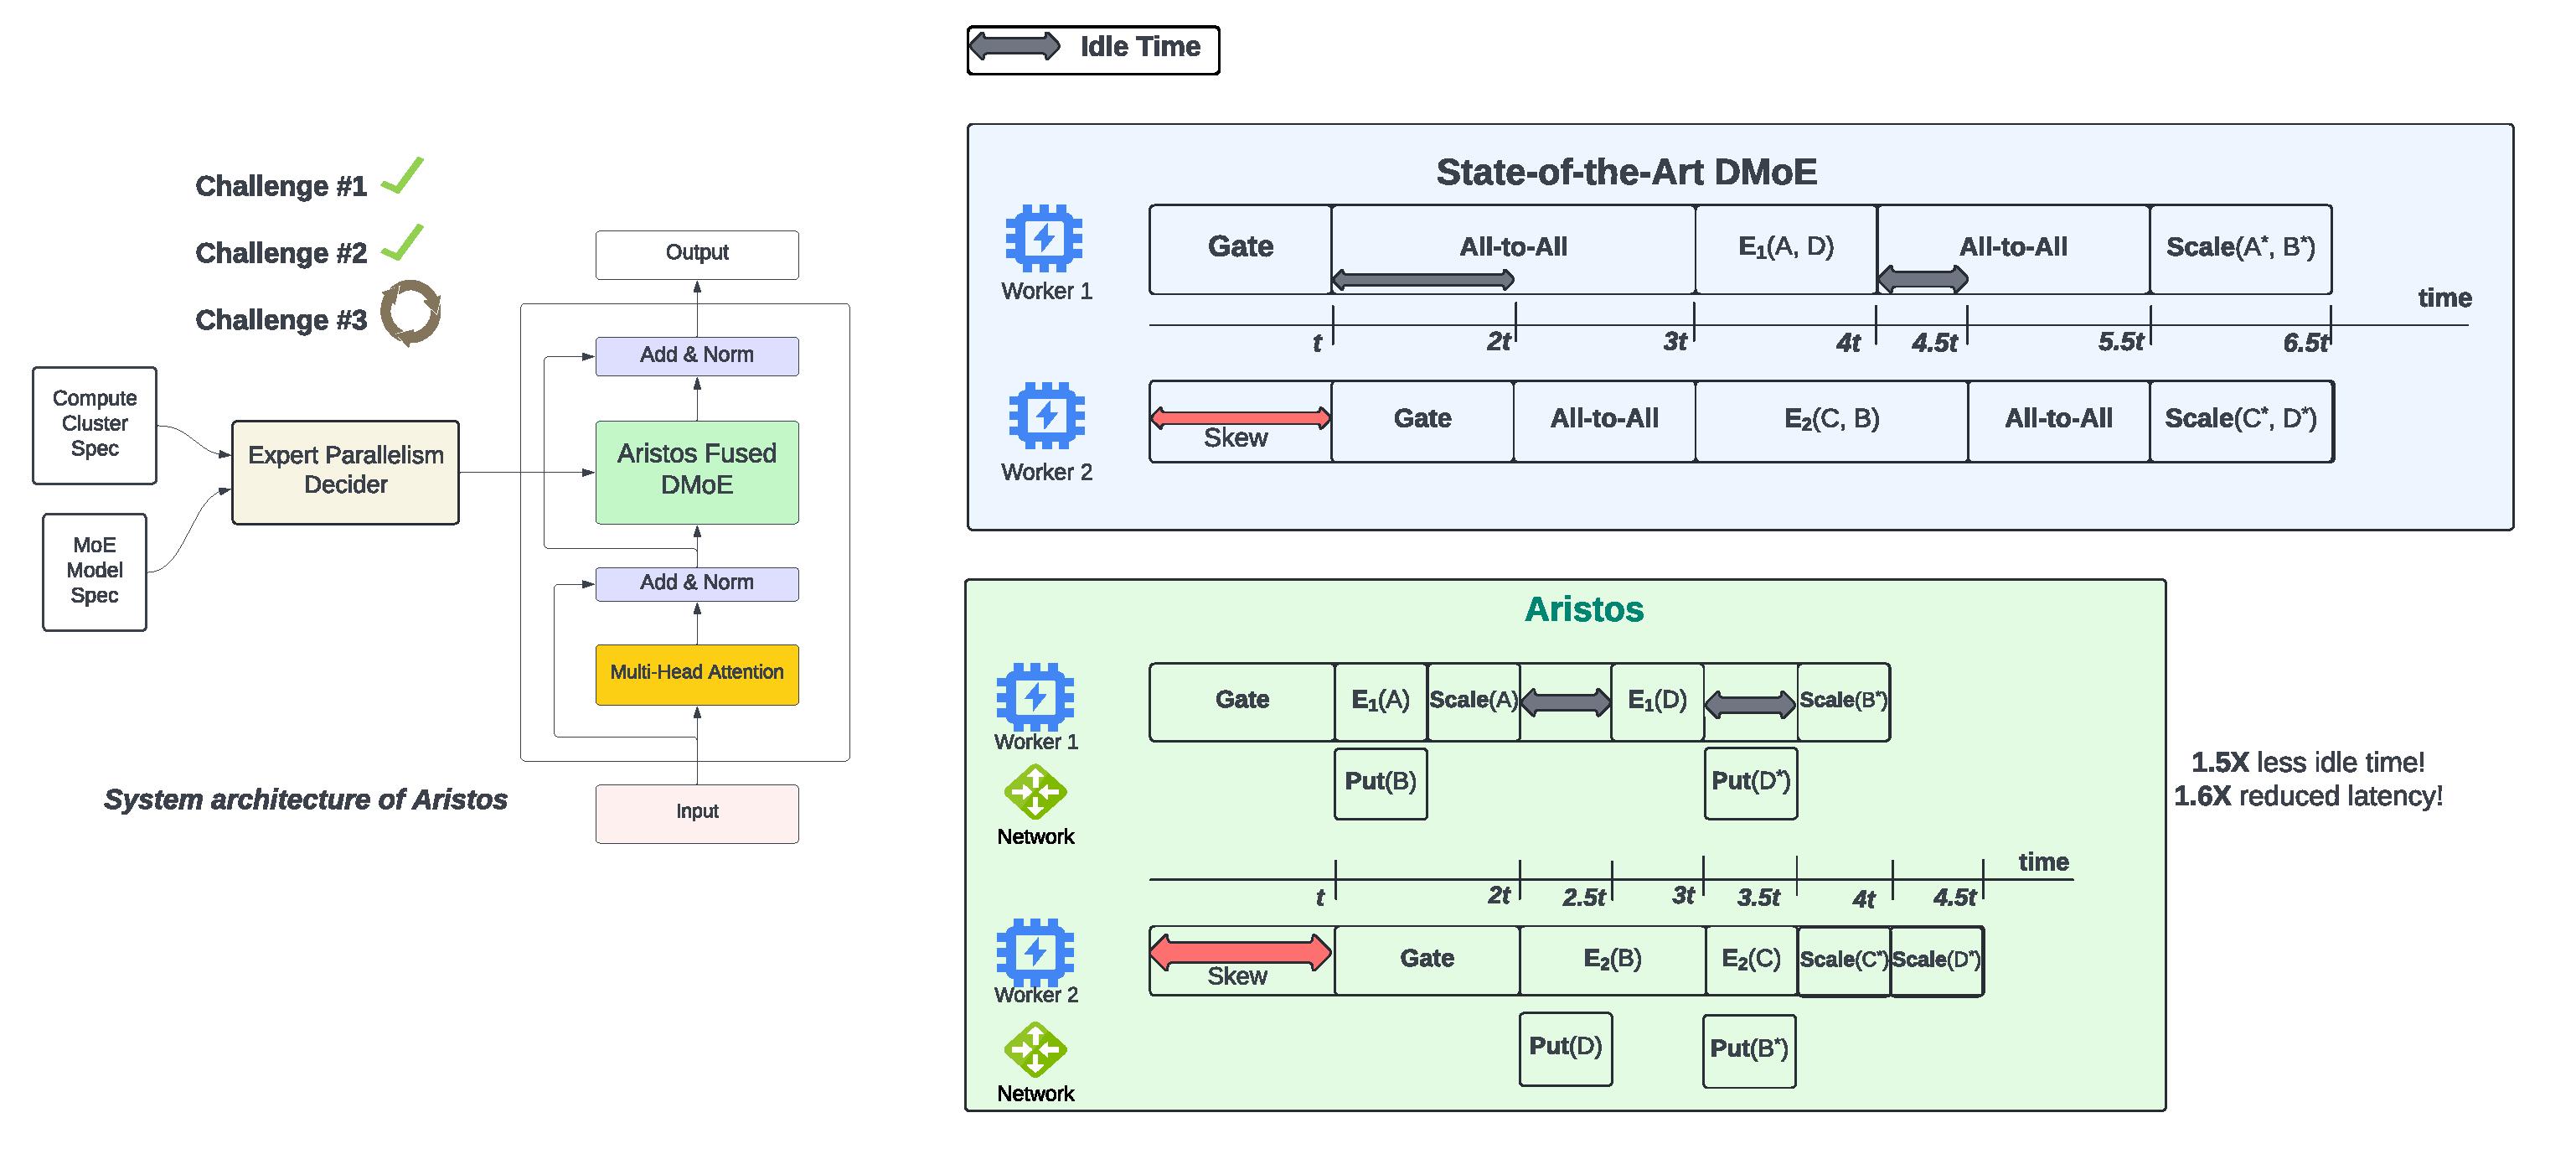
\includegraphics[width=22cm,keepaspectratio]{figures/Aristos_case_1}
            \end{center}
        }

        \headerbox{Microbenchmarks}{name=micro,span=2,column=0, below=method}{
            \begin{center}
                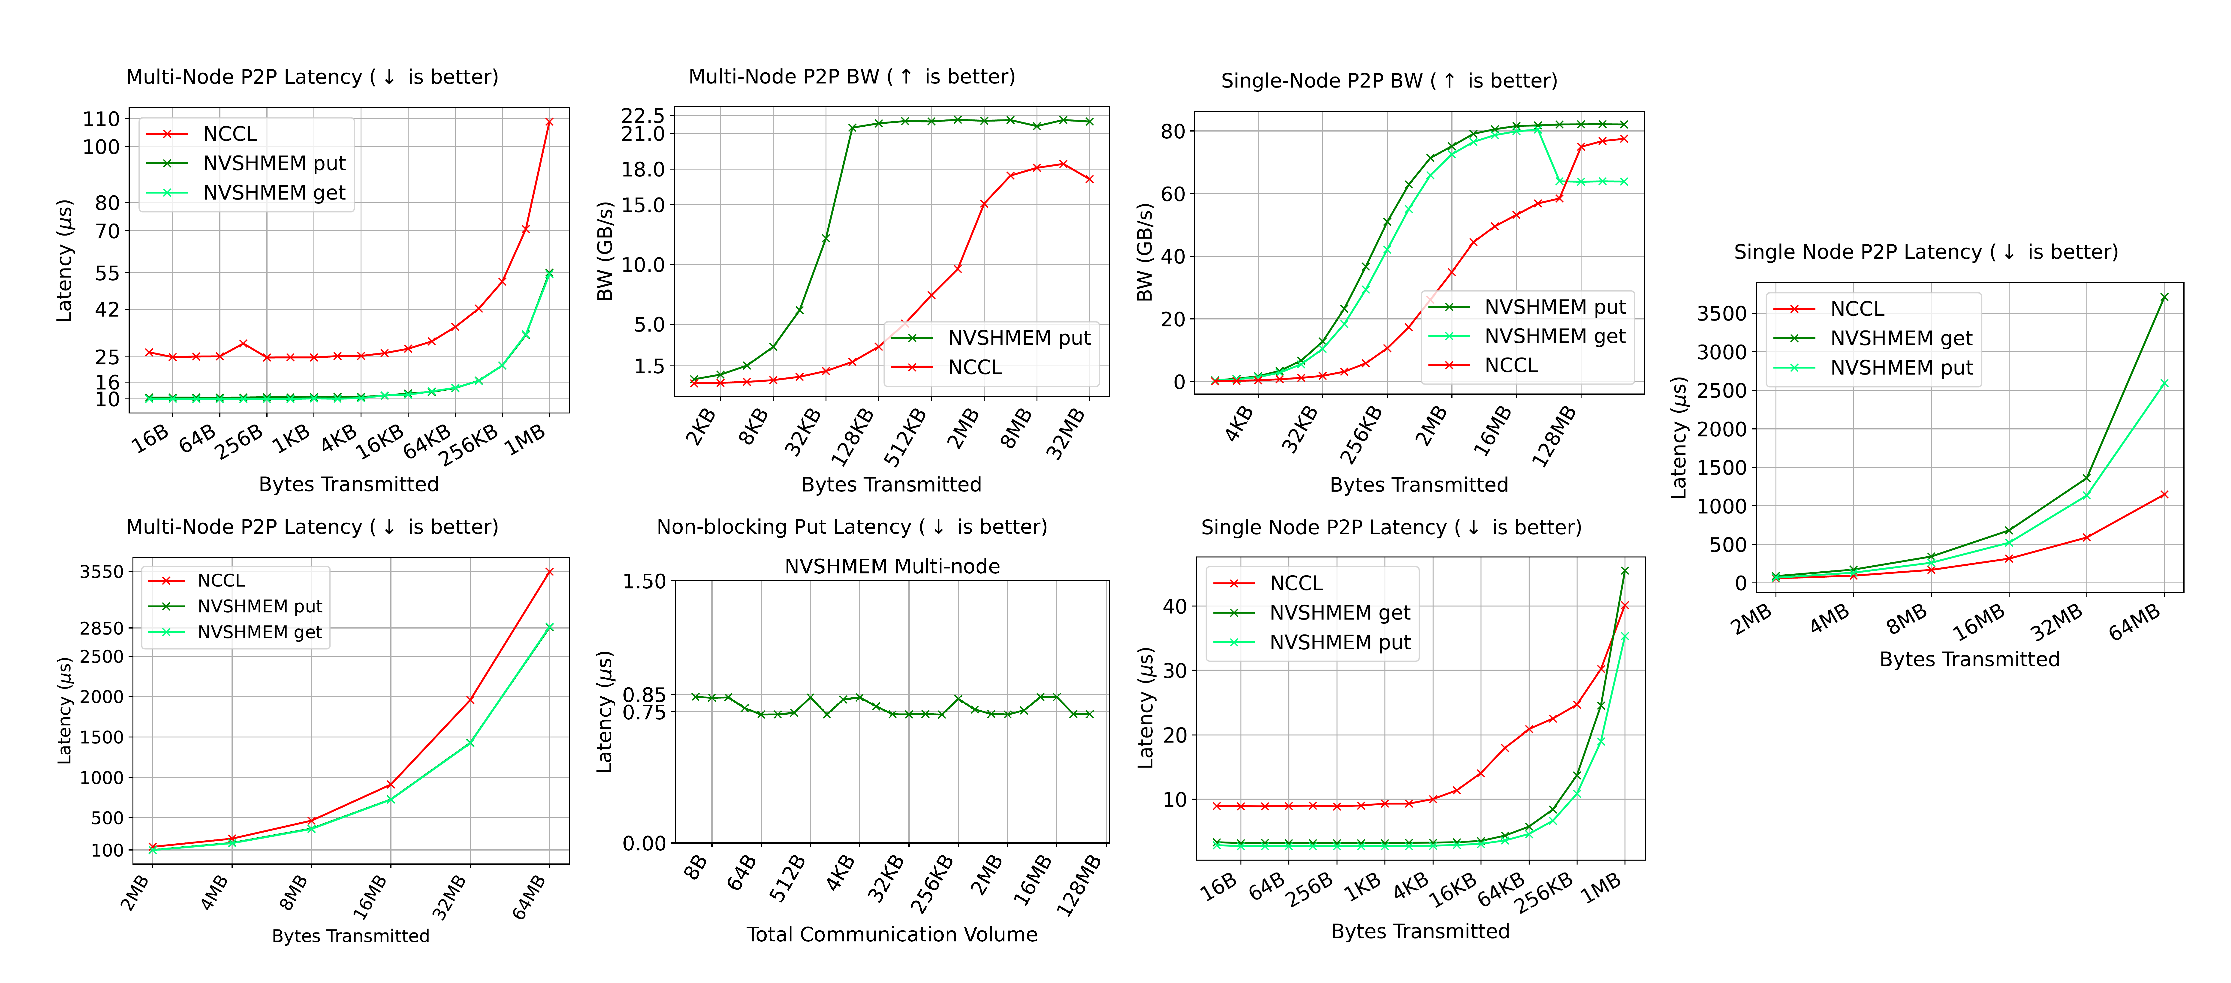
\includegraphics[width=15.45cm,keepaspectratio]{figures/nvsh_nccl}
            \end{center}
        }

        \headerbox{Acknowledgements}{name=ack,span=1, column=2,  below=method}{
            \small{We thank Dr. Rachee Singh for her guidance; Dr. Guila Guidi for Perlmutter access
            under award DDR-ERCAP0027296 of the
            National Energy Research Scientific Computing Center (NERSC); and Julian Bellavita
            for invigorating discussions.}
        }

        \headerbox{References}{name=references,span=1, column=2,  below=ack}{
            \printbibliography[heading=none]
        }

    \end{poster}
\end{document}
